\section{Anexo - Arquitectura}

En el presente anexo se documenta la arquitectura de software de la plataforma \textbf{SocioUnido} utilizando el modelo C4. Este modelo permite visualizar el sistema desde distintos niveles de abstracción, facilitando la comprensión tanto para perfiles técnicos de desarrollo y operaciones, como para perfiles de negocio.

A continuación, se presentan los diagramas correspondientes a los niveles de Contexto (Nivel 1), Contenedores (Nivel 2) y Componentes (Nivel 3) para los distintos microservicios que componen el ecosistema.

\subsection{Nivel 1 del modelo de arquitectura C4}

\begin{figure}[h!]
    \centering
    
\includegraphics[width=0.85\textwidth]{img/c4_model/C4 Nivel 1.png}
    \caption{Diagrama C4 nivel 1: Contexto del sistema. Interacción de la plataforma SocioUnido con los distintos actores (Socios, Dirigencia, Personal de Control) y sistemas externos (Pasarela de Pagos, Interfaz de Programación de Aplicaciones [API] de WhatsApp).}
    \label{fig:c4_nivel1}
\end{figure}

\newpage

\subsection{Nivel 2 del modelo de arquitectura C4}

\begin{figure}[h!]
    \centering
    
\includegraphics[width=\textwidth]{img/c4_model/C4 Nivel 2.png}
    \caption{Diagrama C4 nivel 2: Contenedores. Vista de alto nivel de las aplicaciones web, móviles, bases de datos y la arquitectura basada en microservicios detrás de la puerta de enlace de API (API Gateway).}
    \label{fig:c4_nivel2}
\end{figure}

\newpage

\subsection{Nivel 3 del modelo de arquitectura C4}

\subsubsection{Microservicio central (Core)}

\begin{figure}[h!]
    \centering
    
\includegraphics[width=0.9\textwidth]{img/c4_model/C4 Nivel 3-MS Gestion.png}
    \caption{Diagrama C4 nivel 3: Componentes (Microservicio de gestión societaria). Detalle del microservicio principal encargado del CRUD de usuarios, perfiles y reglas de negocio del padrón societario.}
    \label{fig:c4_nivel3_gestion}
\end{figure}

\newpage

\subsubsection{Microservicio de procesamiento de lenguaje natural (PLN)}

\begin{figure}[h!]
    \centering
    
\includegraphics[width=\textwidth]{img/c4_model/C4 Nivel 3-MS NLP.png}
    \caption{Diagrama C4 nivel 3: Componentes (Microservicio de Procesamiento de Lenguaje Natural [PLN]). Detalle del motor integrado vía Webhook con la API de WhatsApp.}
    \label{fig:c4_nivel3_nlp}
\end{figure}

\newpage

\subsubsection{Microservicio de pagos}

\begin{figure}[h!]
    \centering
    
\includegraphics[width=0.85\textwidth]{img/c4_model/C4 Nivel 3-MS Payments.png}
    \caption{Diagrama C4 nivel 3: Componentes (Microservicio de pagos). Arquitectura del componente encargado de la facturación automatizada y comunicación externa con pasarelas.}
    \label{fig:c4_nivel3_payments}
\end{figure}

\newpage

\subsubsection{Microservicio de acceso inteligente}

\begin{figure}[h!]
    \centering
    
\includegraphics[width=0.6\textwidth]{img/c4_model/C4 Nivel 3-MS Smart Access.png} % Asumiendo nombre acorde a la versión anterior, ajustar de ser necesario.
    \caption{Diagrama C4 nivel 3: Componentes (Microservicio de acceso inteligente). Lógica interna de validación matemática mediante TOTP para el control de accesos en estadios.}
    \label{fig:c4_nivel3_smartaccess}
\end{figure}

\newpage

\subsubsection{Microservicio de autenticación}

\begin{figure}[h!]
    \centering
    
\includegraphics[width=\textwidth]{img/c4_model/C4 Nivel 3-MS Auth.png}
    \caption{Diagrama C4 nivel 3: Componentes (Microservicio de autenticación). Sistema para el manejo seguro de identidades y generación de tokens JWT.}
    \label{fig:c4_nivel3_auth}
\end{figure}

\newpage

\subsubsection{Microservicio de analítica e inteligencia artificial}

\begin{figure}[h!]
    \centering
    
\includegraphics[width=0.6\textwidth]{img/c4_model/C4 Nivel 3-MS Analytics & AI.png}
    \caption{Diagrama C4 nivel 3: Componentes (Microservicio de analítica e inteligencia artificial). Orquestación de tareas asíncronas y motor de Machine Learning.}
    \label{fig:c4_nivel3_analytics}
\end{figure}

\newpage

\subsubsection{Gateway}

\begin{figure}[h!]
    \centering
    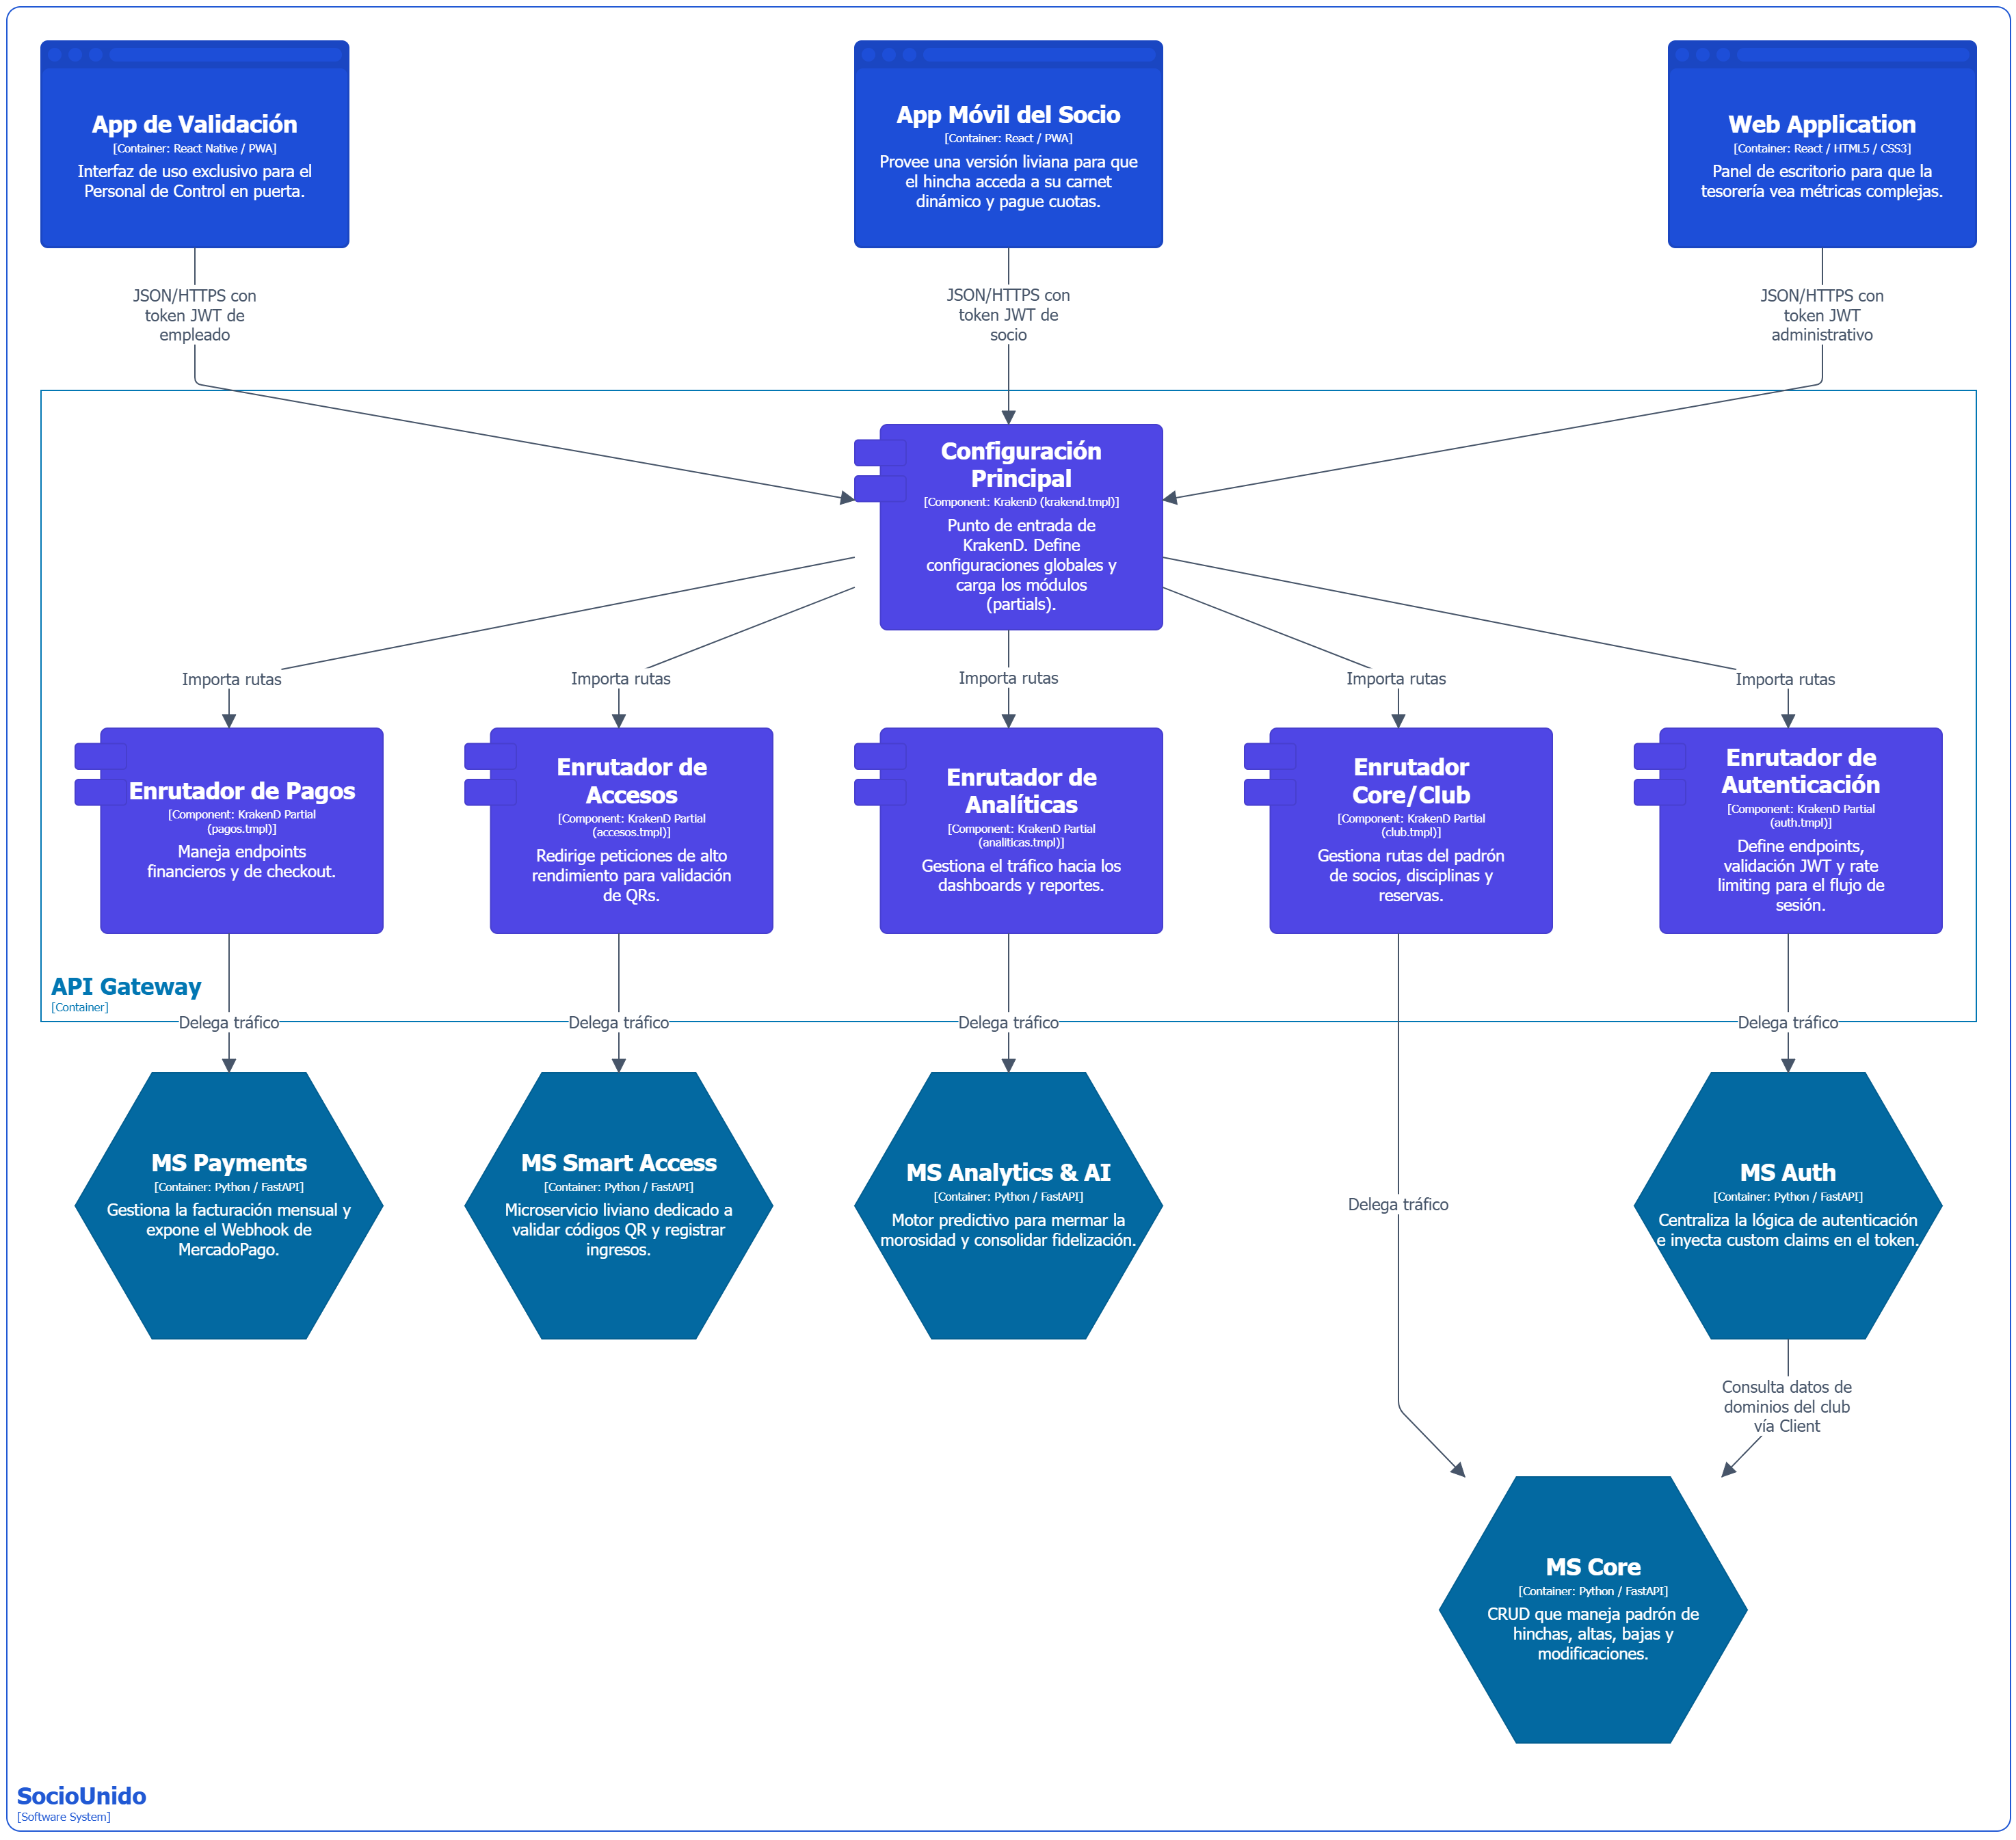
\includegraphics[width=\textwidth]{img/c4_model/C4 Nivel 3-Gateway.png}
    \caption{Diagrama C4 nivel 3: Componentes (API Gateway). Punto de entrada unificado basado en KrakenD, encargado de interceptar peticiones, validar tokens JWT, aplicar limitación de tasa (Rate Limiting) y enrutar el tráfico hacia los microservicios correspondientes.}
    \label{fig:c4_nivel3_gateway}
\end{figure}

\newpage

\subsubsection{Web administrativa (Panel de gestión)}

\begin{figure}[h!]
    \centering
    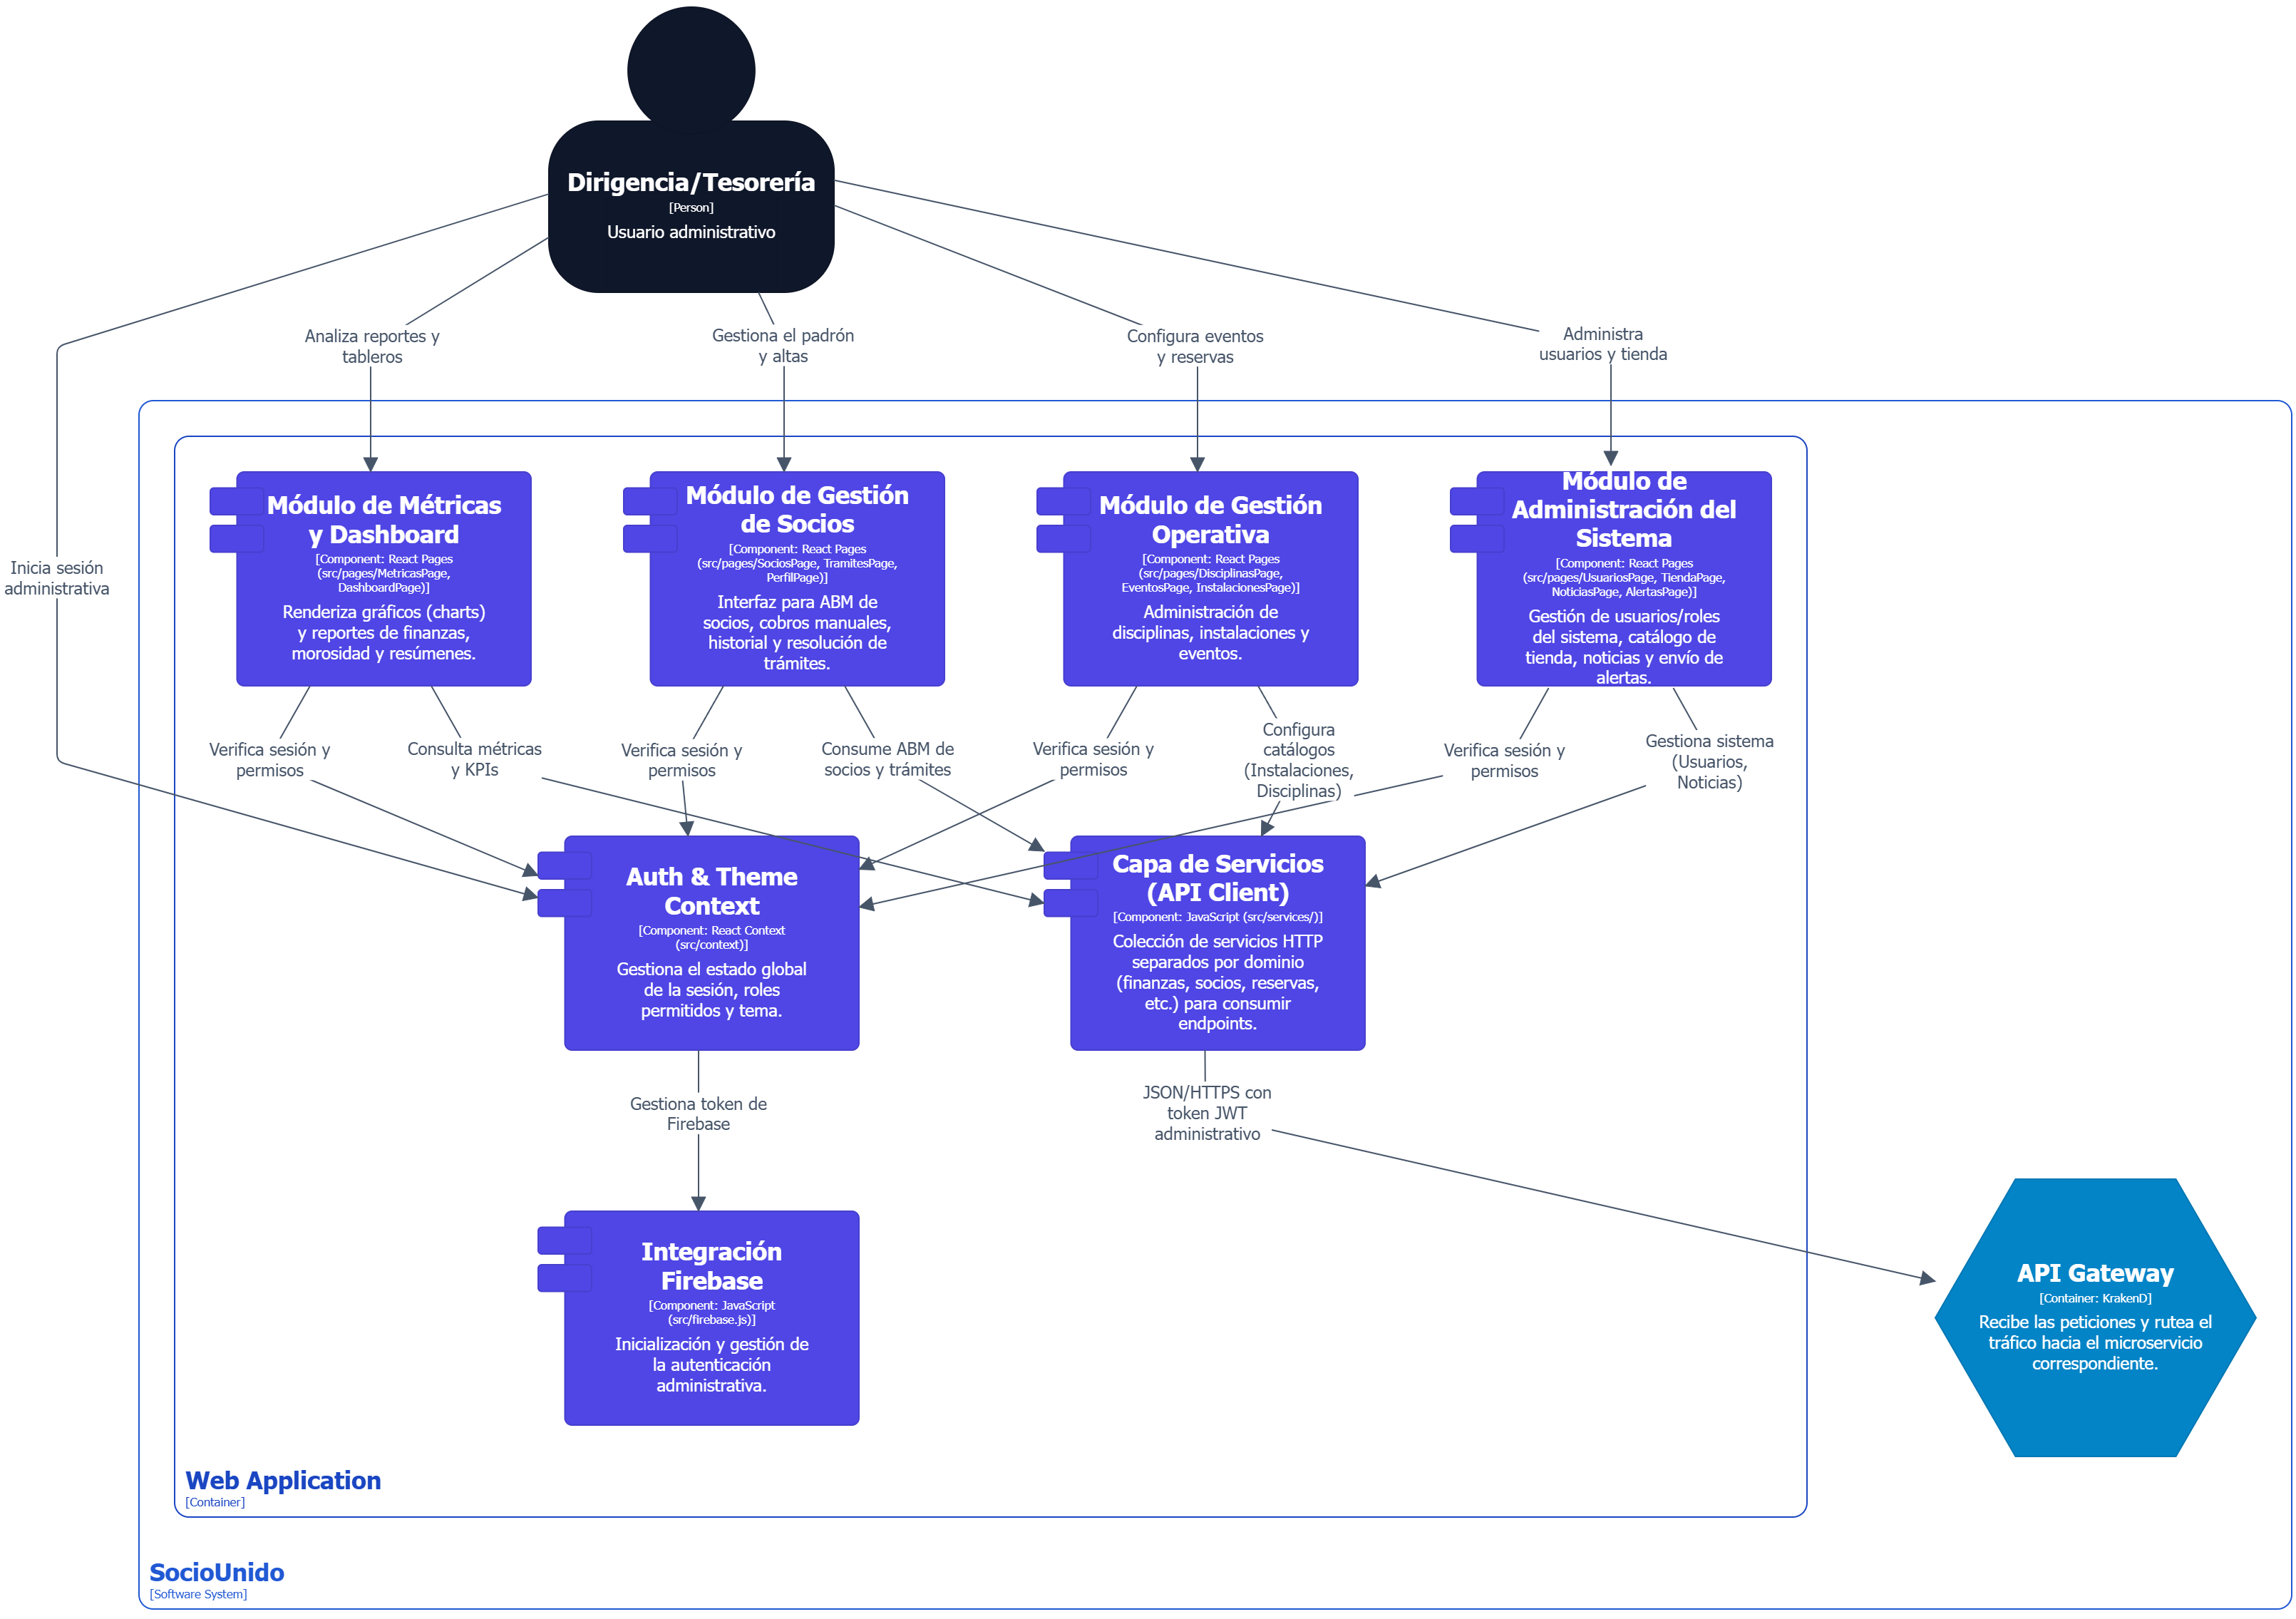
\includegraphics[width=\textwidth]{img/c4_model/C4 Nivel 3-Web Administrativa.png} % Ajustado de .jpg a .png según carpeta
    \caption{Diagrama C4 nivel 3: Componentes (Web administrativa). Aplicación frontend orientada al personal del club, que centraliza la administración de socios, disciplinas, reservas e informes.}
    \label{fig:c4_nivel3_webadmin}
\end{figure}

\newpage

\subsubsection{App del Socio (PWA)}

\begin{figure}[h!]
    \centering
    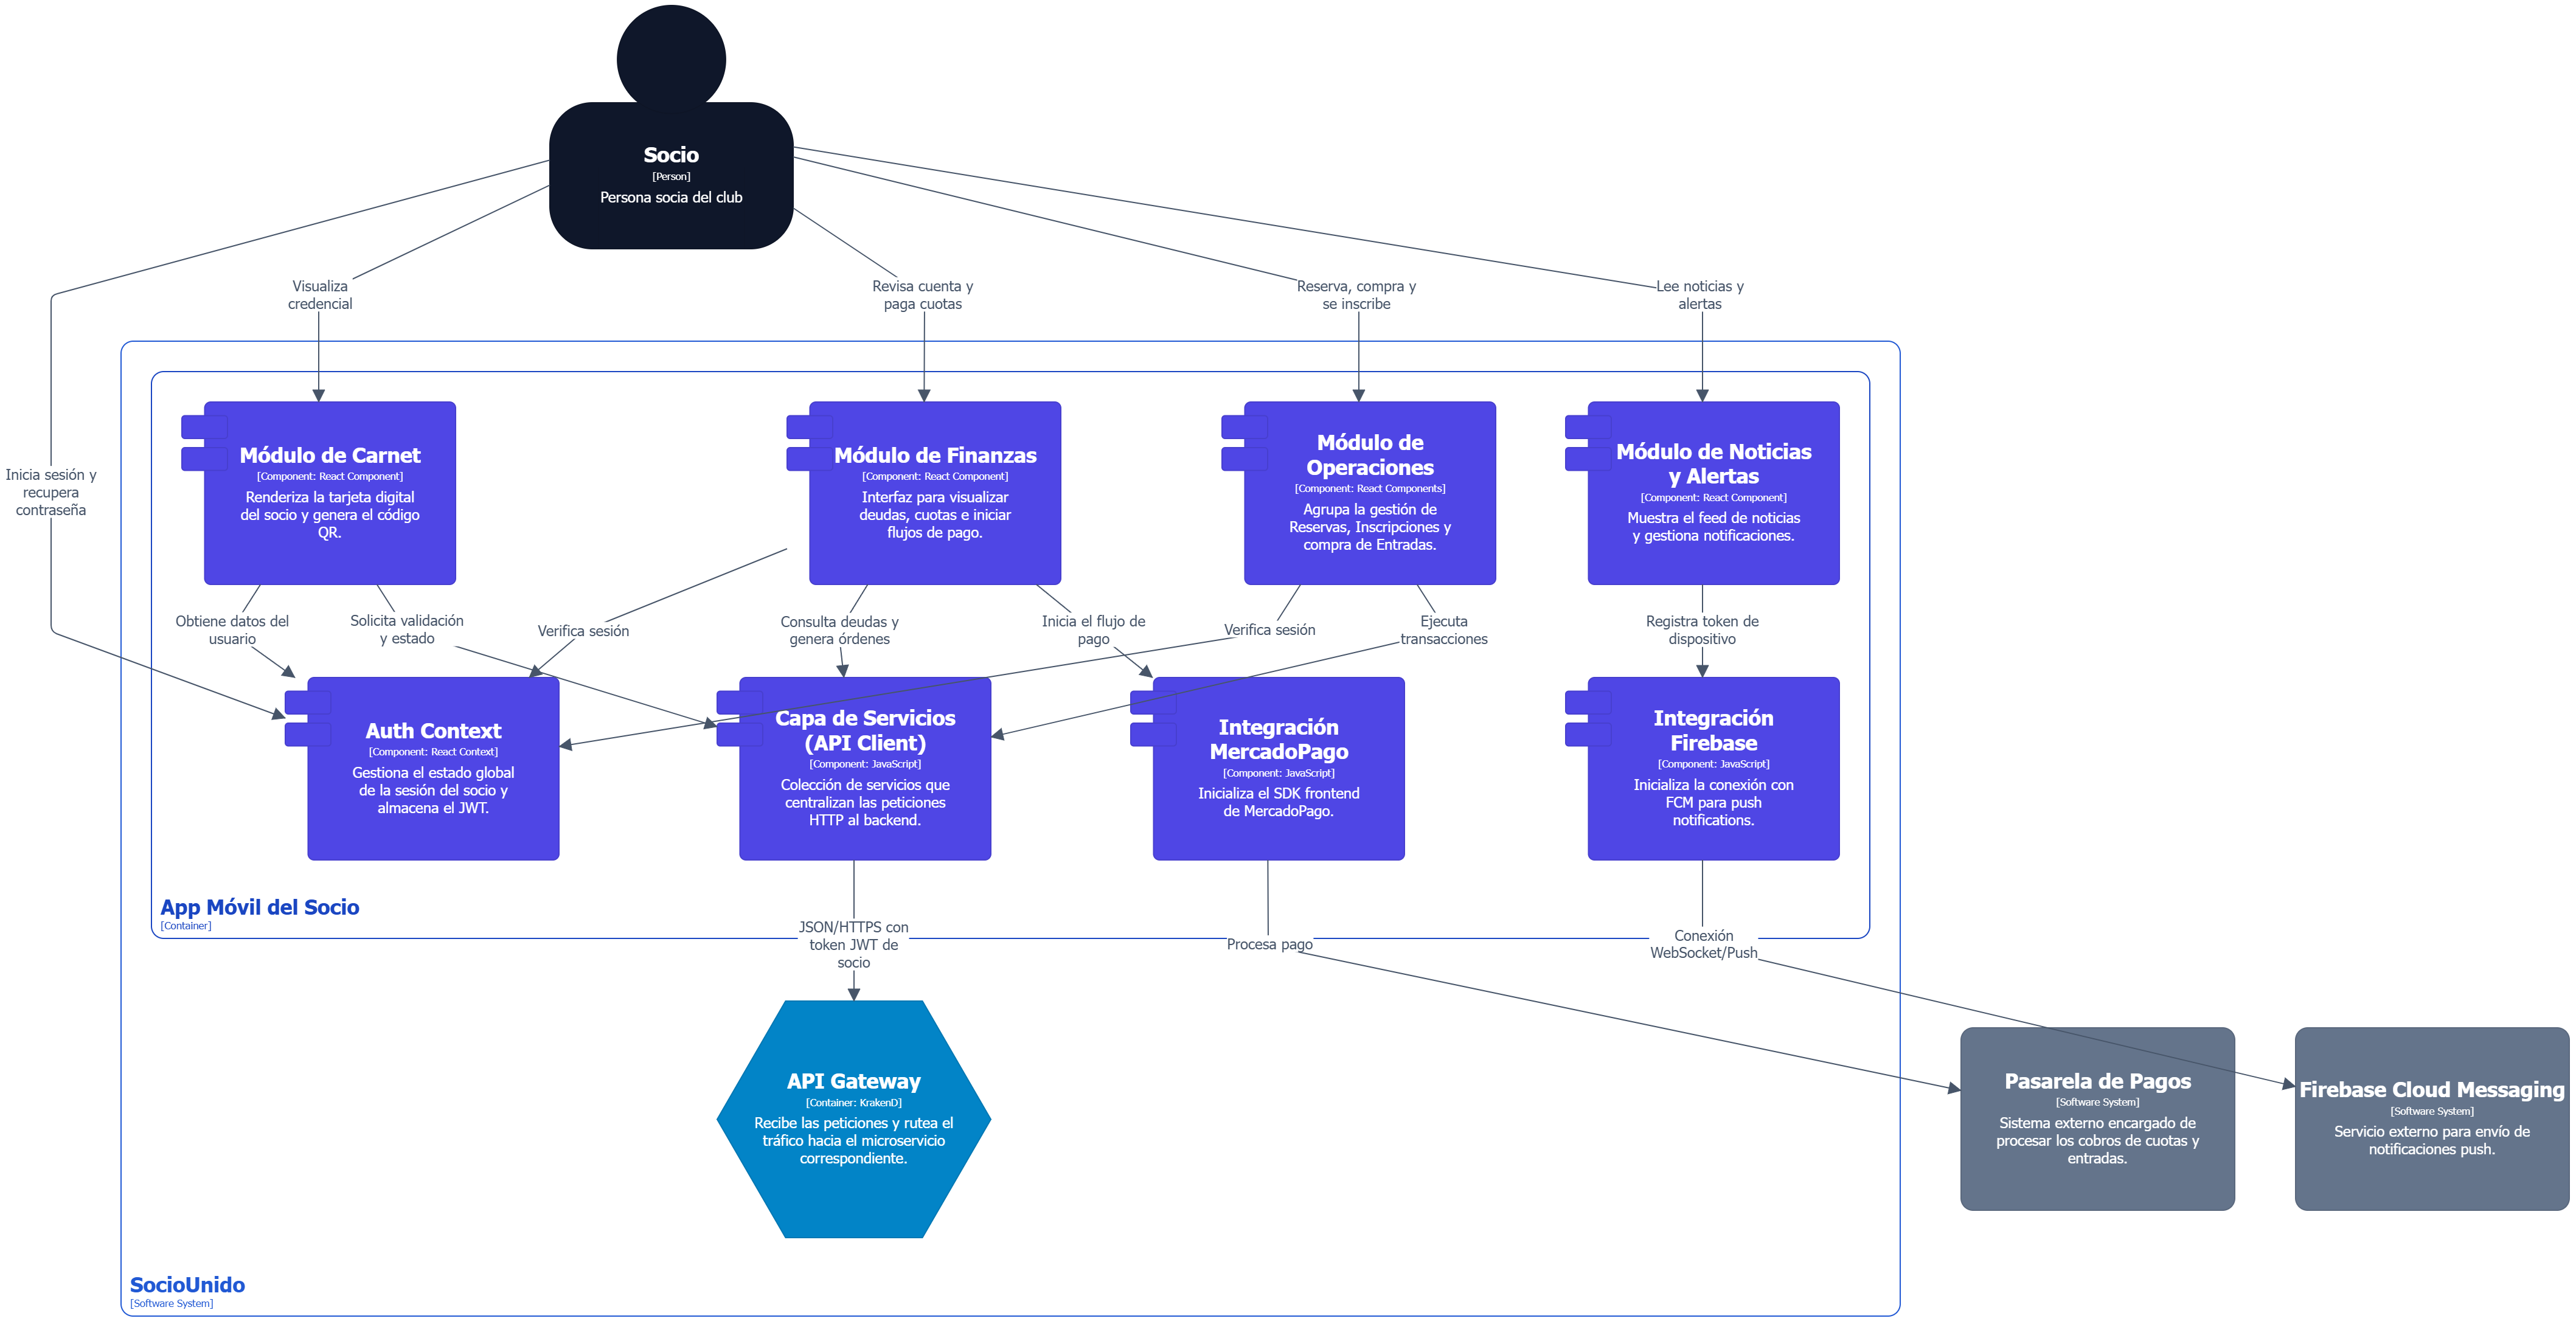
\includegraphics[width=\textwidth]{img/c4_model/C4 Nivel 3-App Socio.png}
    \caption{Diagrama C4 nivel 3: Componentes (App del Socio [PWA]). Aplicación Web Progresiva diseñada para el usuario final, con soporte offline y notificaciones push.}
    \label{fig:c4_nivel3_appsocio}
\end{figure}

\subsubsection{App del Empleado (PWA)}

\begin{figure}[h!]
    \centering
    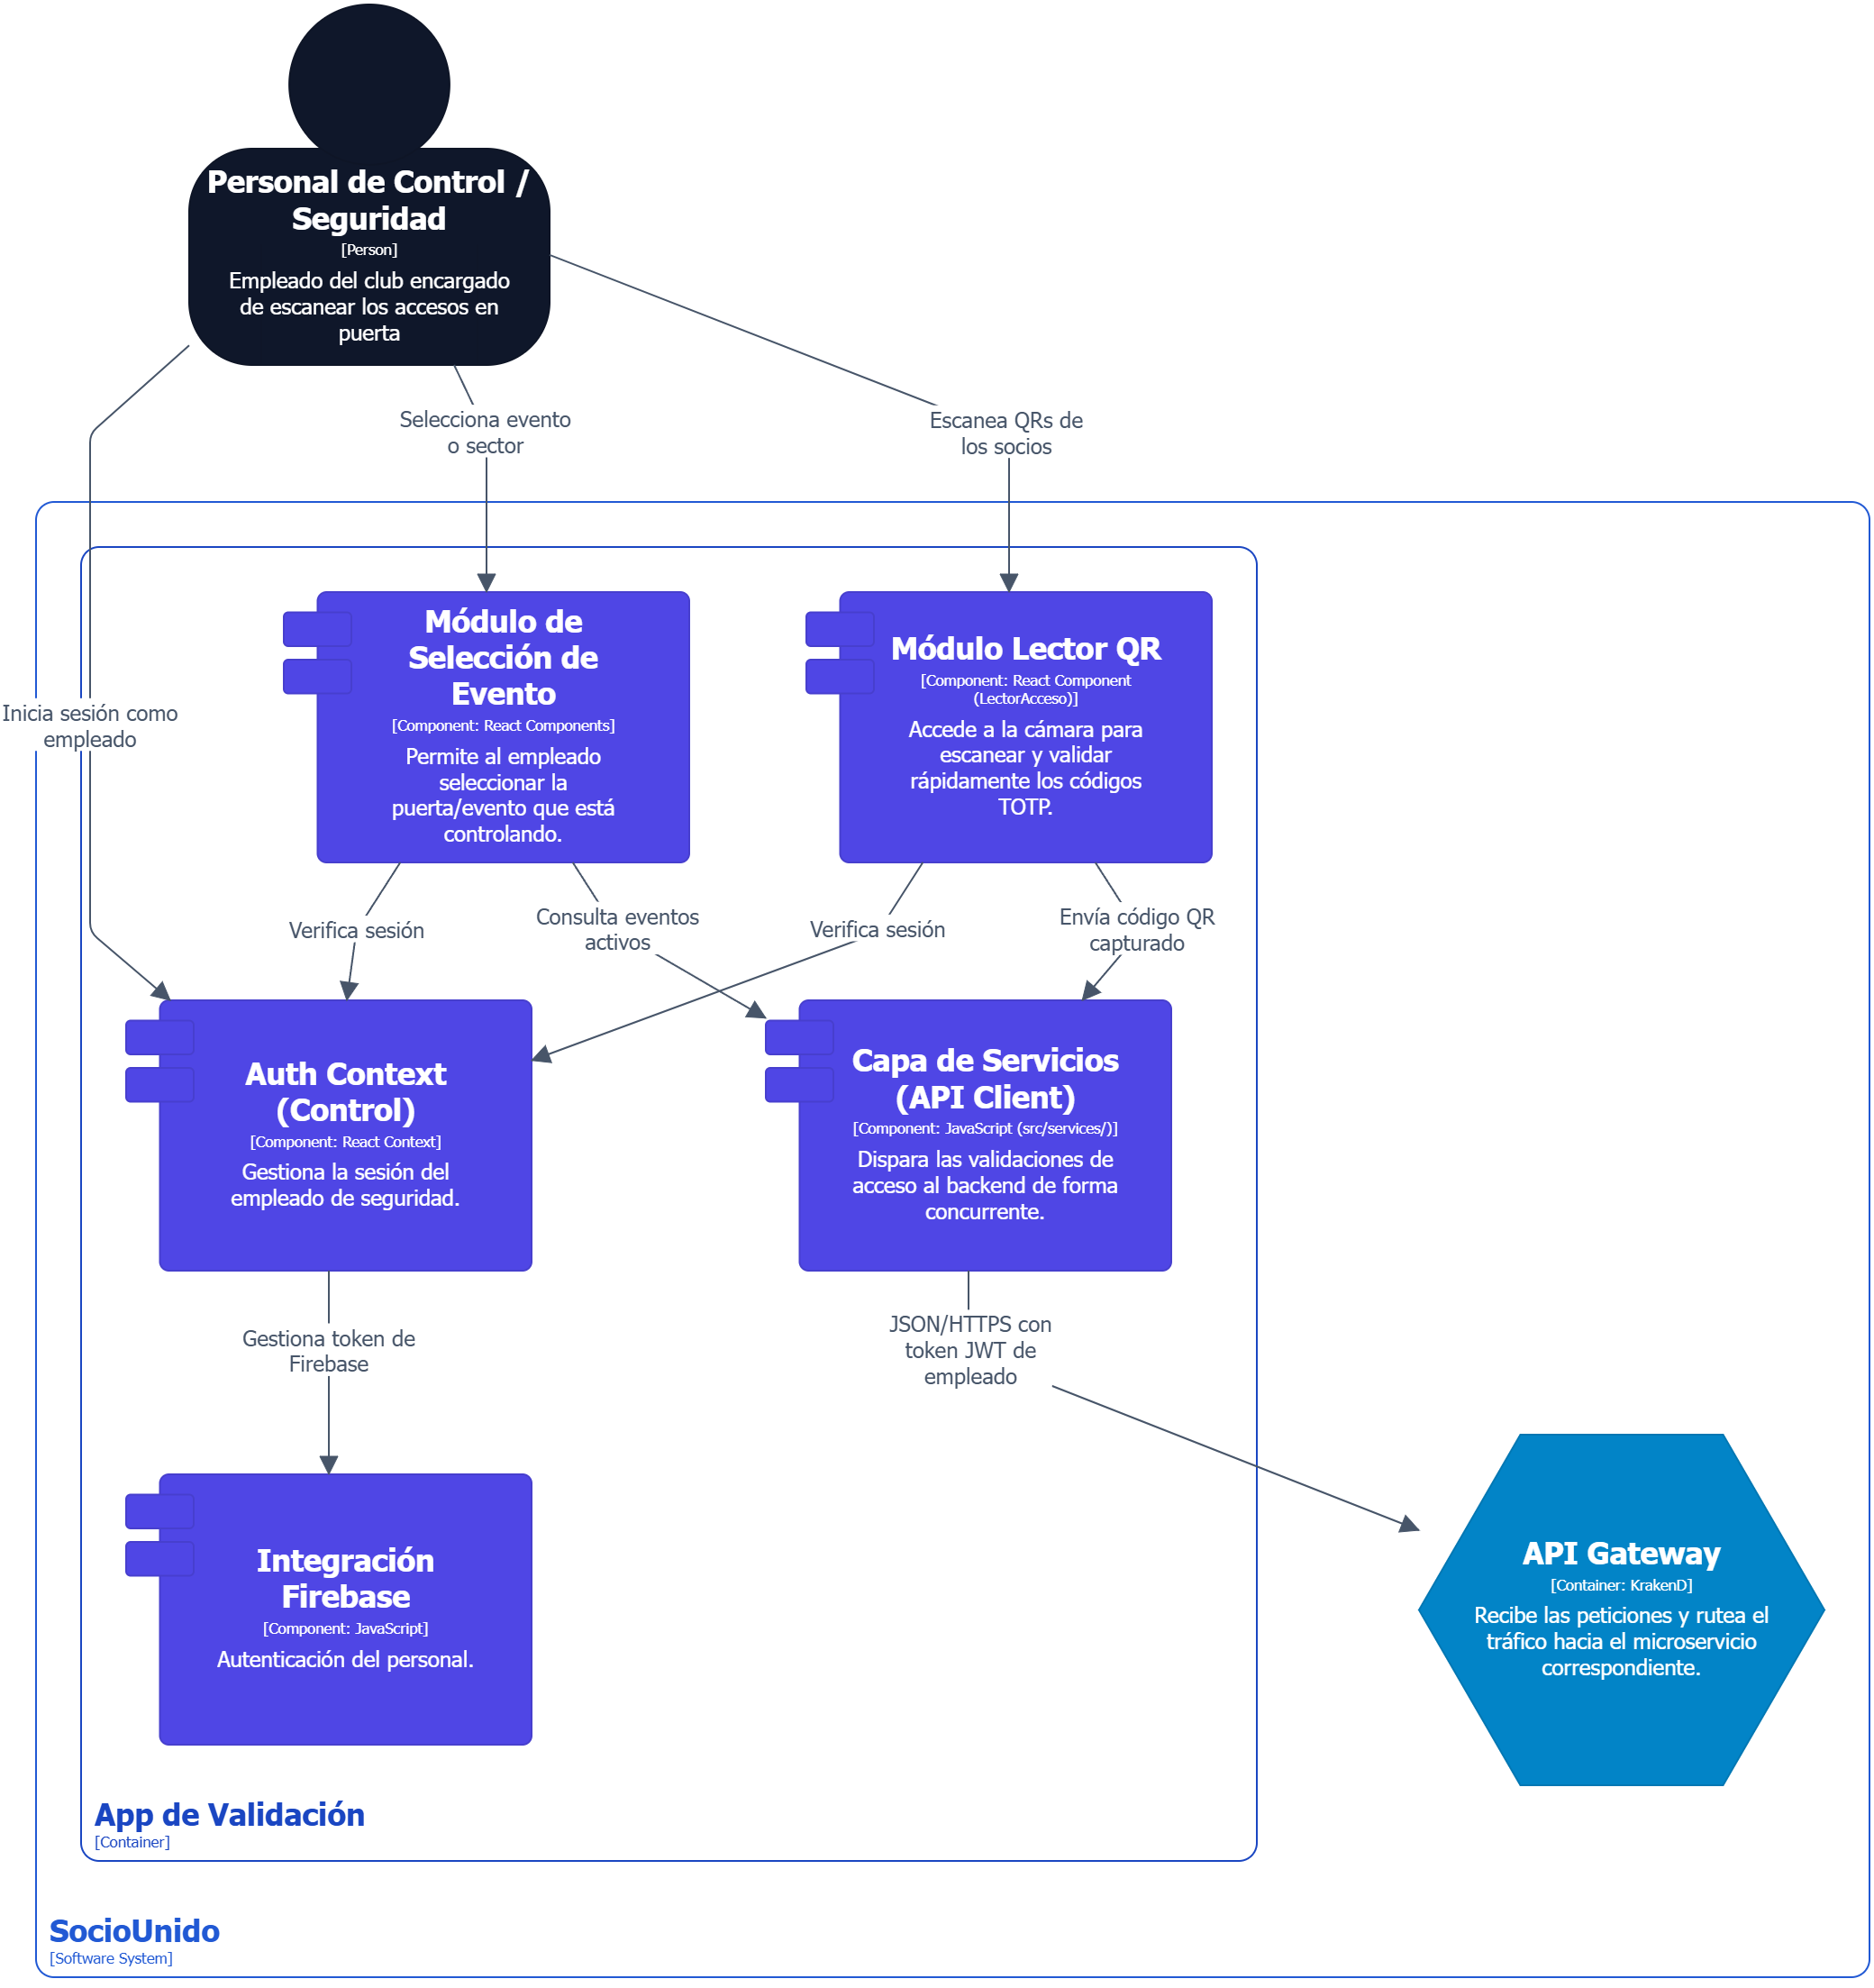
\includegraphics[width=0.6\textwidth]{img/c4_model/C4 Nivel 3- App Empleados.png}
    \caption{Diagrama C4 nivel 3: Componentes (App del Empleado [PWA]). Aplicación orientada al personal operativo y de campo del club, enfocada en la gestión y control de ingresos.}
    \label{fig:c4_nivel3_appempleados}
\end{figure}

\newpage

\subsection{Monitoreo y resiliencia: Servicio de Healthchecker}

Para garantizar la alta disponibilidad, observabilidad y resiliencia del ecosistema de \textbf{SocioUnido}, se ha incorporado un nodo dedicado exclusivamente al monitoreo continuo del sistema: el \textbf{Servicio de Healthchecker}. 

\subsubsection*{Justificación Técnica y Arquitectónica}
En arquitecturas distribuidas basadas en microservicios, la degradación o falla parcial de un componente no debe comprometer la integridad global de la plataforma ni pasar desapercibida. El patrón de \textit{Health Check} implementado mediante un nodo observador independiente permite aislar la lógica de monitoreo del flujo principal de datos (como el API Gateway o los microservicios de negocio centrales). 

El diseño y propósito de este nodo abarca los siguientes puntos críticos:
\begin{itemize}
    \item \textbf{Monitoreo Activo (Pull-based):} Realiza rutinas programadas de verificación (pings HTTP/TCP) consultando los \textit{endpoints} de salud designados (típicamente \texttt{/health} o \texttt{/metrics}) en cada uno de los microservicios y bases de datos.
    \item \textbf{Evaluación de Latencia y Estado de Salud:} Además de validar la correcta recepción de códigos HTTP \texttt{200 OK}, el sistema actúa como una sonda que mide los tiempos de respuesta. Esto permite detectar bloqueos de base de datos, cuellos de botella en la red o degradación progresiva del rendimiento antes de que decante en una interrupción total del servicio (\textit{Downtime}).
    \item \textbf{Auto-recuperación (Self-healing) y Orquestación de Alertas:} Al detectar una caída (cambio de estado de \textit{UP} a \textit{DOWN}), \textit{timeouts} excesivos o anomalías estructurales, el motor de monitoreo está diseñado para actuar proactivamente. Puede ejecutar rutinas de mitigación e interactuar con la infraestructura para reiniciar contenedores comprometidos, o disparar alertas críticas mediante \textit{webhooks} para notificar al equipo en tiempo real.
\end{itemize}

Desacoplar este componente es una decisión arquitectónica vital; asegura que bajo escenarios de alta concurrencia o ataques de denegación de servicio (DDoS) donde el API Gateway se encuentre comprometido o bajo estrés, el monitoreo transversal del sistema mantenga su capacidad operativa sin verse ralentizado por el tráfico de los usuarios finales.

\subsubsection*{Interfaz de administración y control financiero (Frontend)}

Para complementar el monitoreo técnico subyacente, el servicio de Healthchecker integra un panel de control interactivo diseñado como el centro de comando unificado para el equipo de SocioUnido. Esta interfaz consolida tanto la telemetría del sistema como la inteligencia de negocio, sirviendo como el punto de monitoreo central para las necesidades de infraestructura compartida (multitenant) y los nodos aislados por club. Sus tareas críticas abarcan:

\begin{itemize}
    \item \textbf{Tablero de estado global (Node Status Dashboard):} Permite visualizar en tiempo real la salud, latencia y disponibilidad de absolutamente todos los nodos del ecosistema SocioUnido, facilitando una respuesta inmediata ante fallos en cualquier despliegue.
    \item \textbf{Auditoría de transacciones y cálculo de comisiones (Fees):} El panel consolida y expone los datos de los volúmenes financieros operados dentro de la aplicación. Al centralizar las ganancias generadas por las transacciones de cada institución, el sistema calcula automáticamente el porcentaje de retribución correspondiente a SocioUnido, según el modelo de negocio de cobro variable transaccional.
    \newpage
    \item \textbf{Módulo de inteligencia financiera y rentabilidad:} Incorpora una herramienta analítica interactiva (tipo 'calculadora') que permite abstraer y proyectar los costos operativos a nivel macro (global) y a nivel micro (por club específico). Permite el ingreso y cruce de variables de egreso (mantenimiento del servicio, alojamiento de microservicios, bases de datos y gastos misceláneos) con los ingresos fijos y variables. Esto faculta al equipo para analizar el rédito actual, los márgenes de ganancia reales y la viabilidad económica de cada uno de los despliegues en producción.
\end{itemize}

\subsubsection{Nivel 3 del modelo de arquitectura C4 (Healthchecker)}

\begin{figure}[h!]
    \centering
    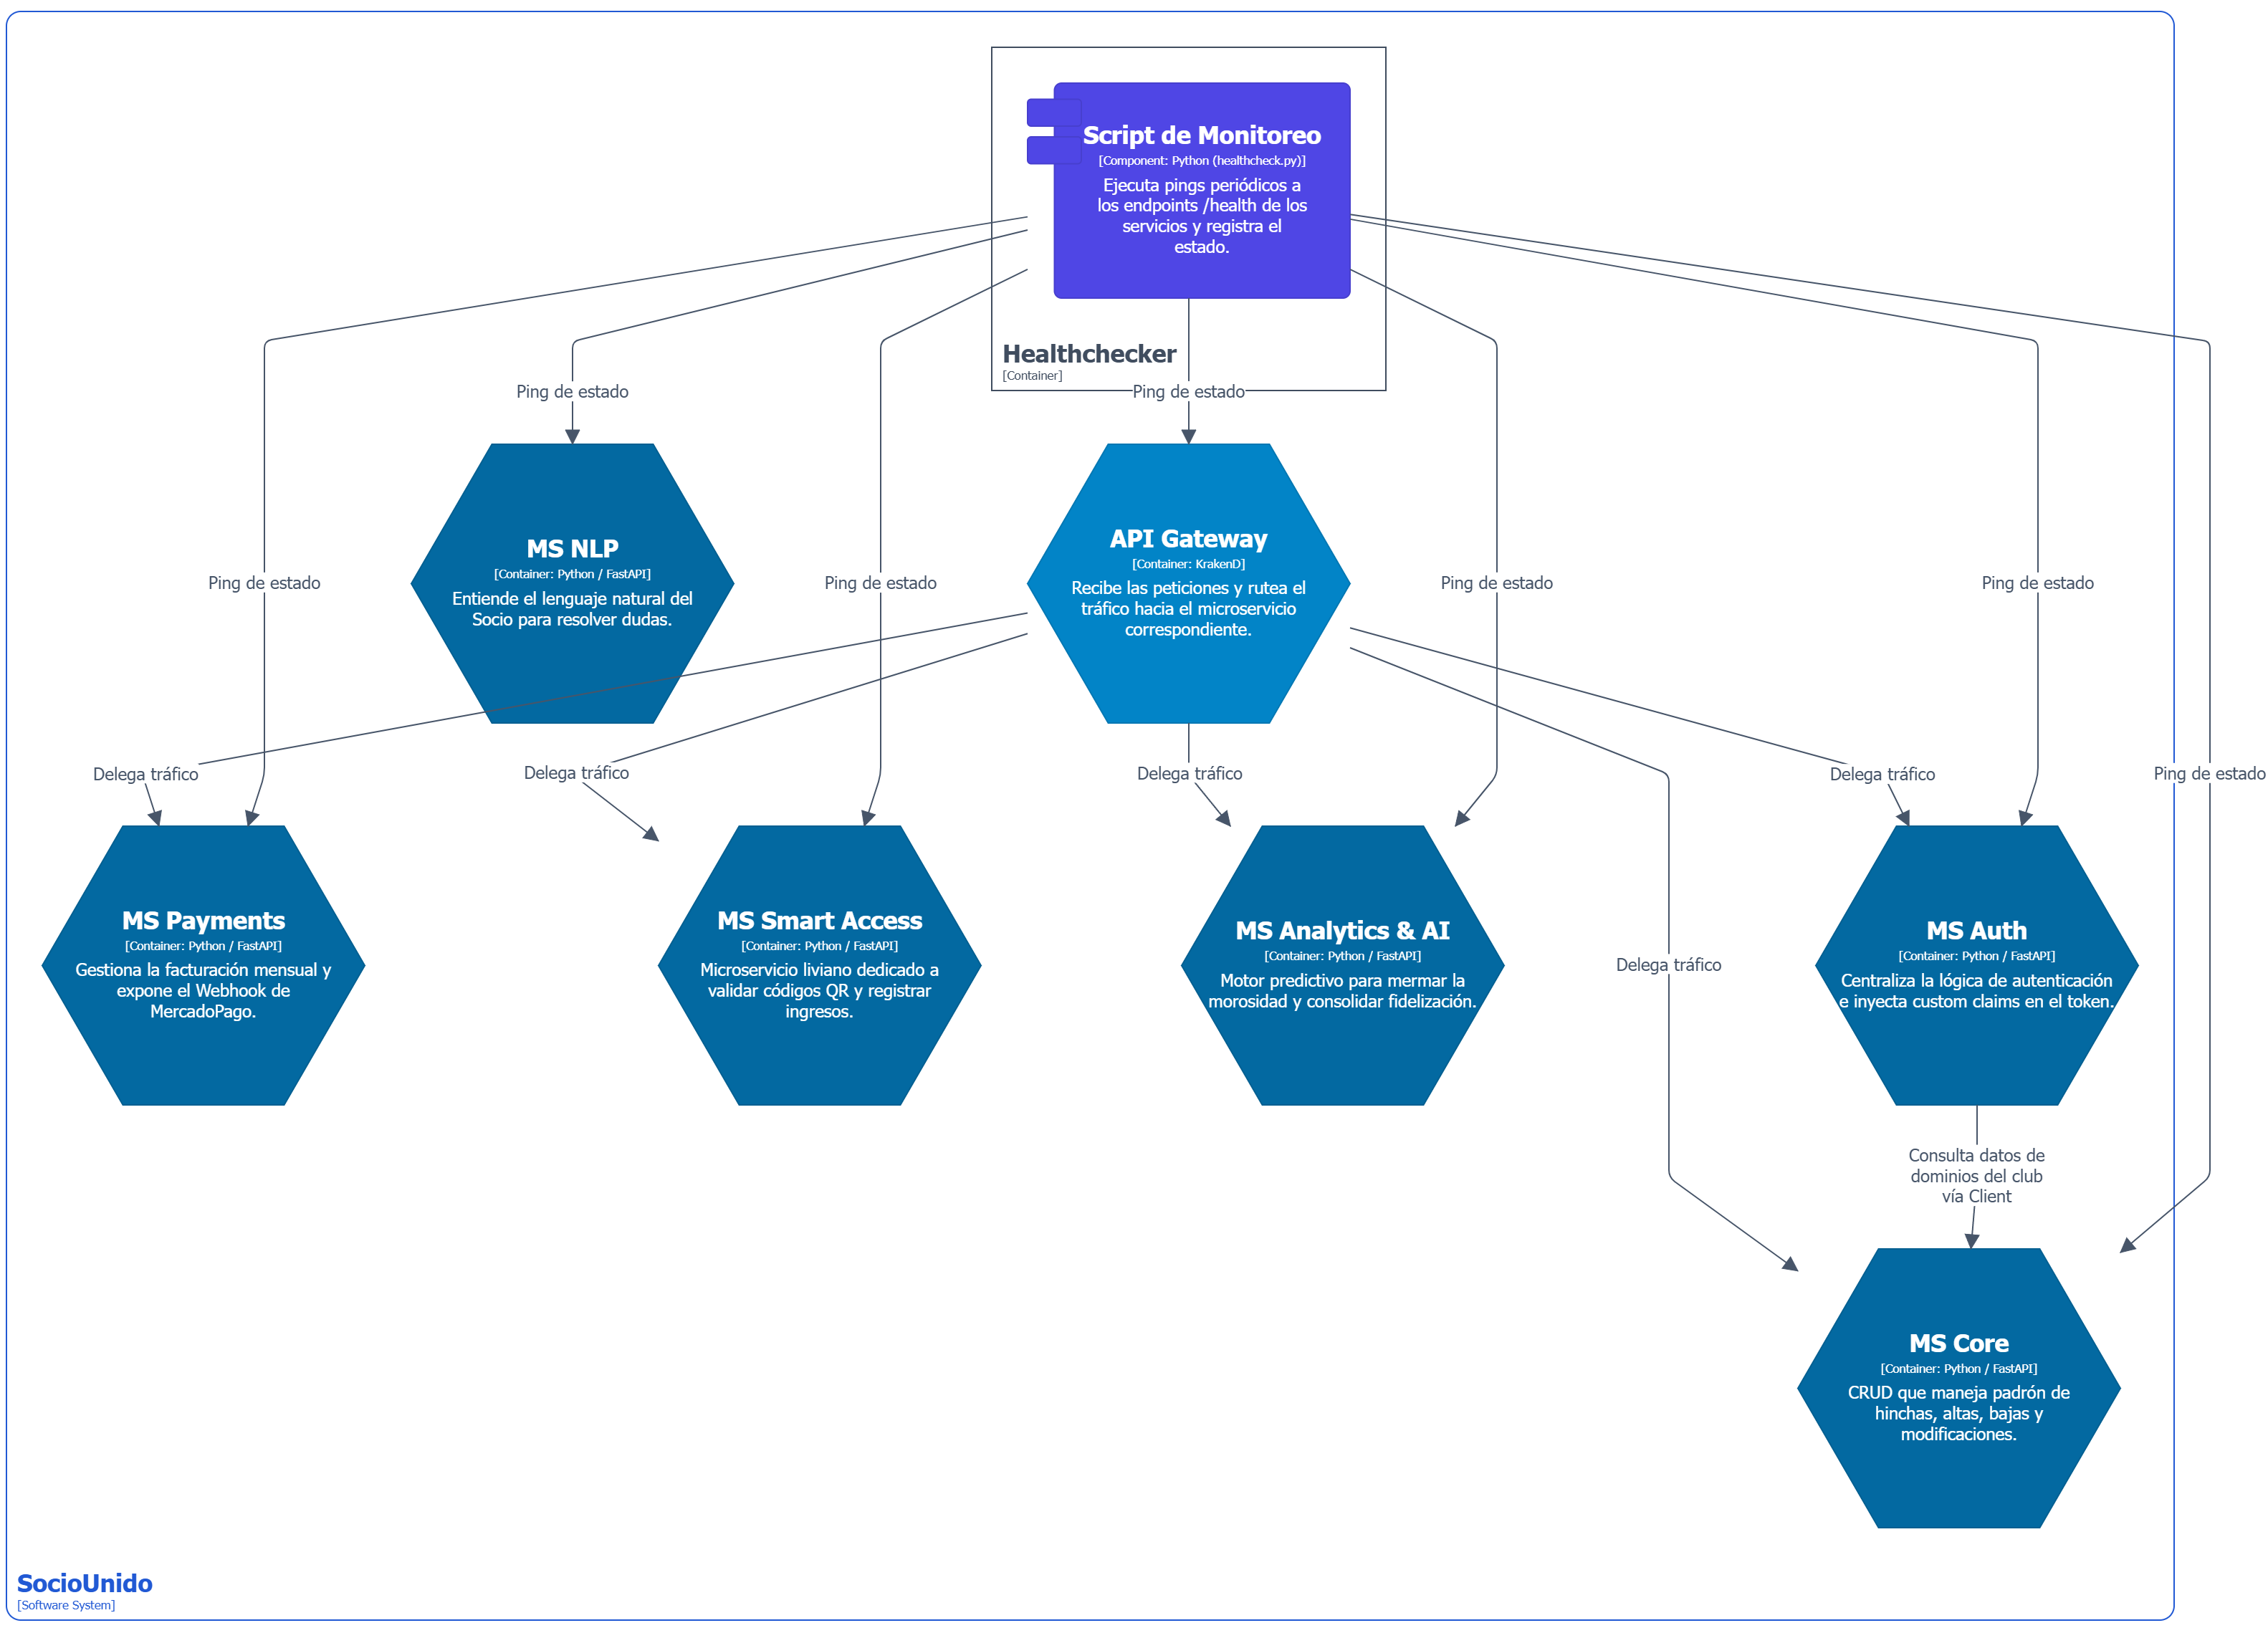
\includegraphics[width=\textwidth]{img/c4_model/C4 Nivel 3- Healthchecker.png}
    \caption{Diagrama C4 nivel 3: Componentes (Healthchecker). Muestra el servicio de observabilidad, monitoreo de disponibilidad (uptime) y bases de datos.}
    \label{fig:healthchecker_c4}
\end{figure}

\newpage

\subsection{Diagramas Entidad-Relación (DER)}

La persistencia del ecosistema de \textbf{SocioUnido} sigue un enfoque descentralizado mediante bases de datos aisladas por microservicio, asegurando la escalabilidad operativa, la consistencia de datos y el principio de responsabilidad única.

A continuación, se detallan las estructuras del modelo relacional para los repositorios de datos principales alojados en la capa de persistencia:

\subsubsection{Base de datos de gestión societaria}
Este esquema relacional centraliza el padrón maestro del club deportivo. Administra la información de contacto de los socios, la asignación de categorías, el control de roles administrativos internos de la dirigencia y las reglas de negocio esenciales de la institución.

\begin{figure}[h!]
    \centering
    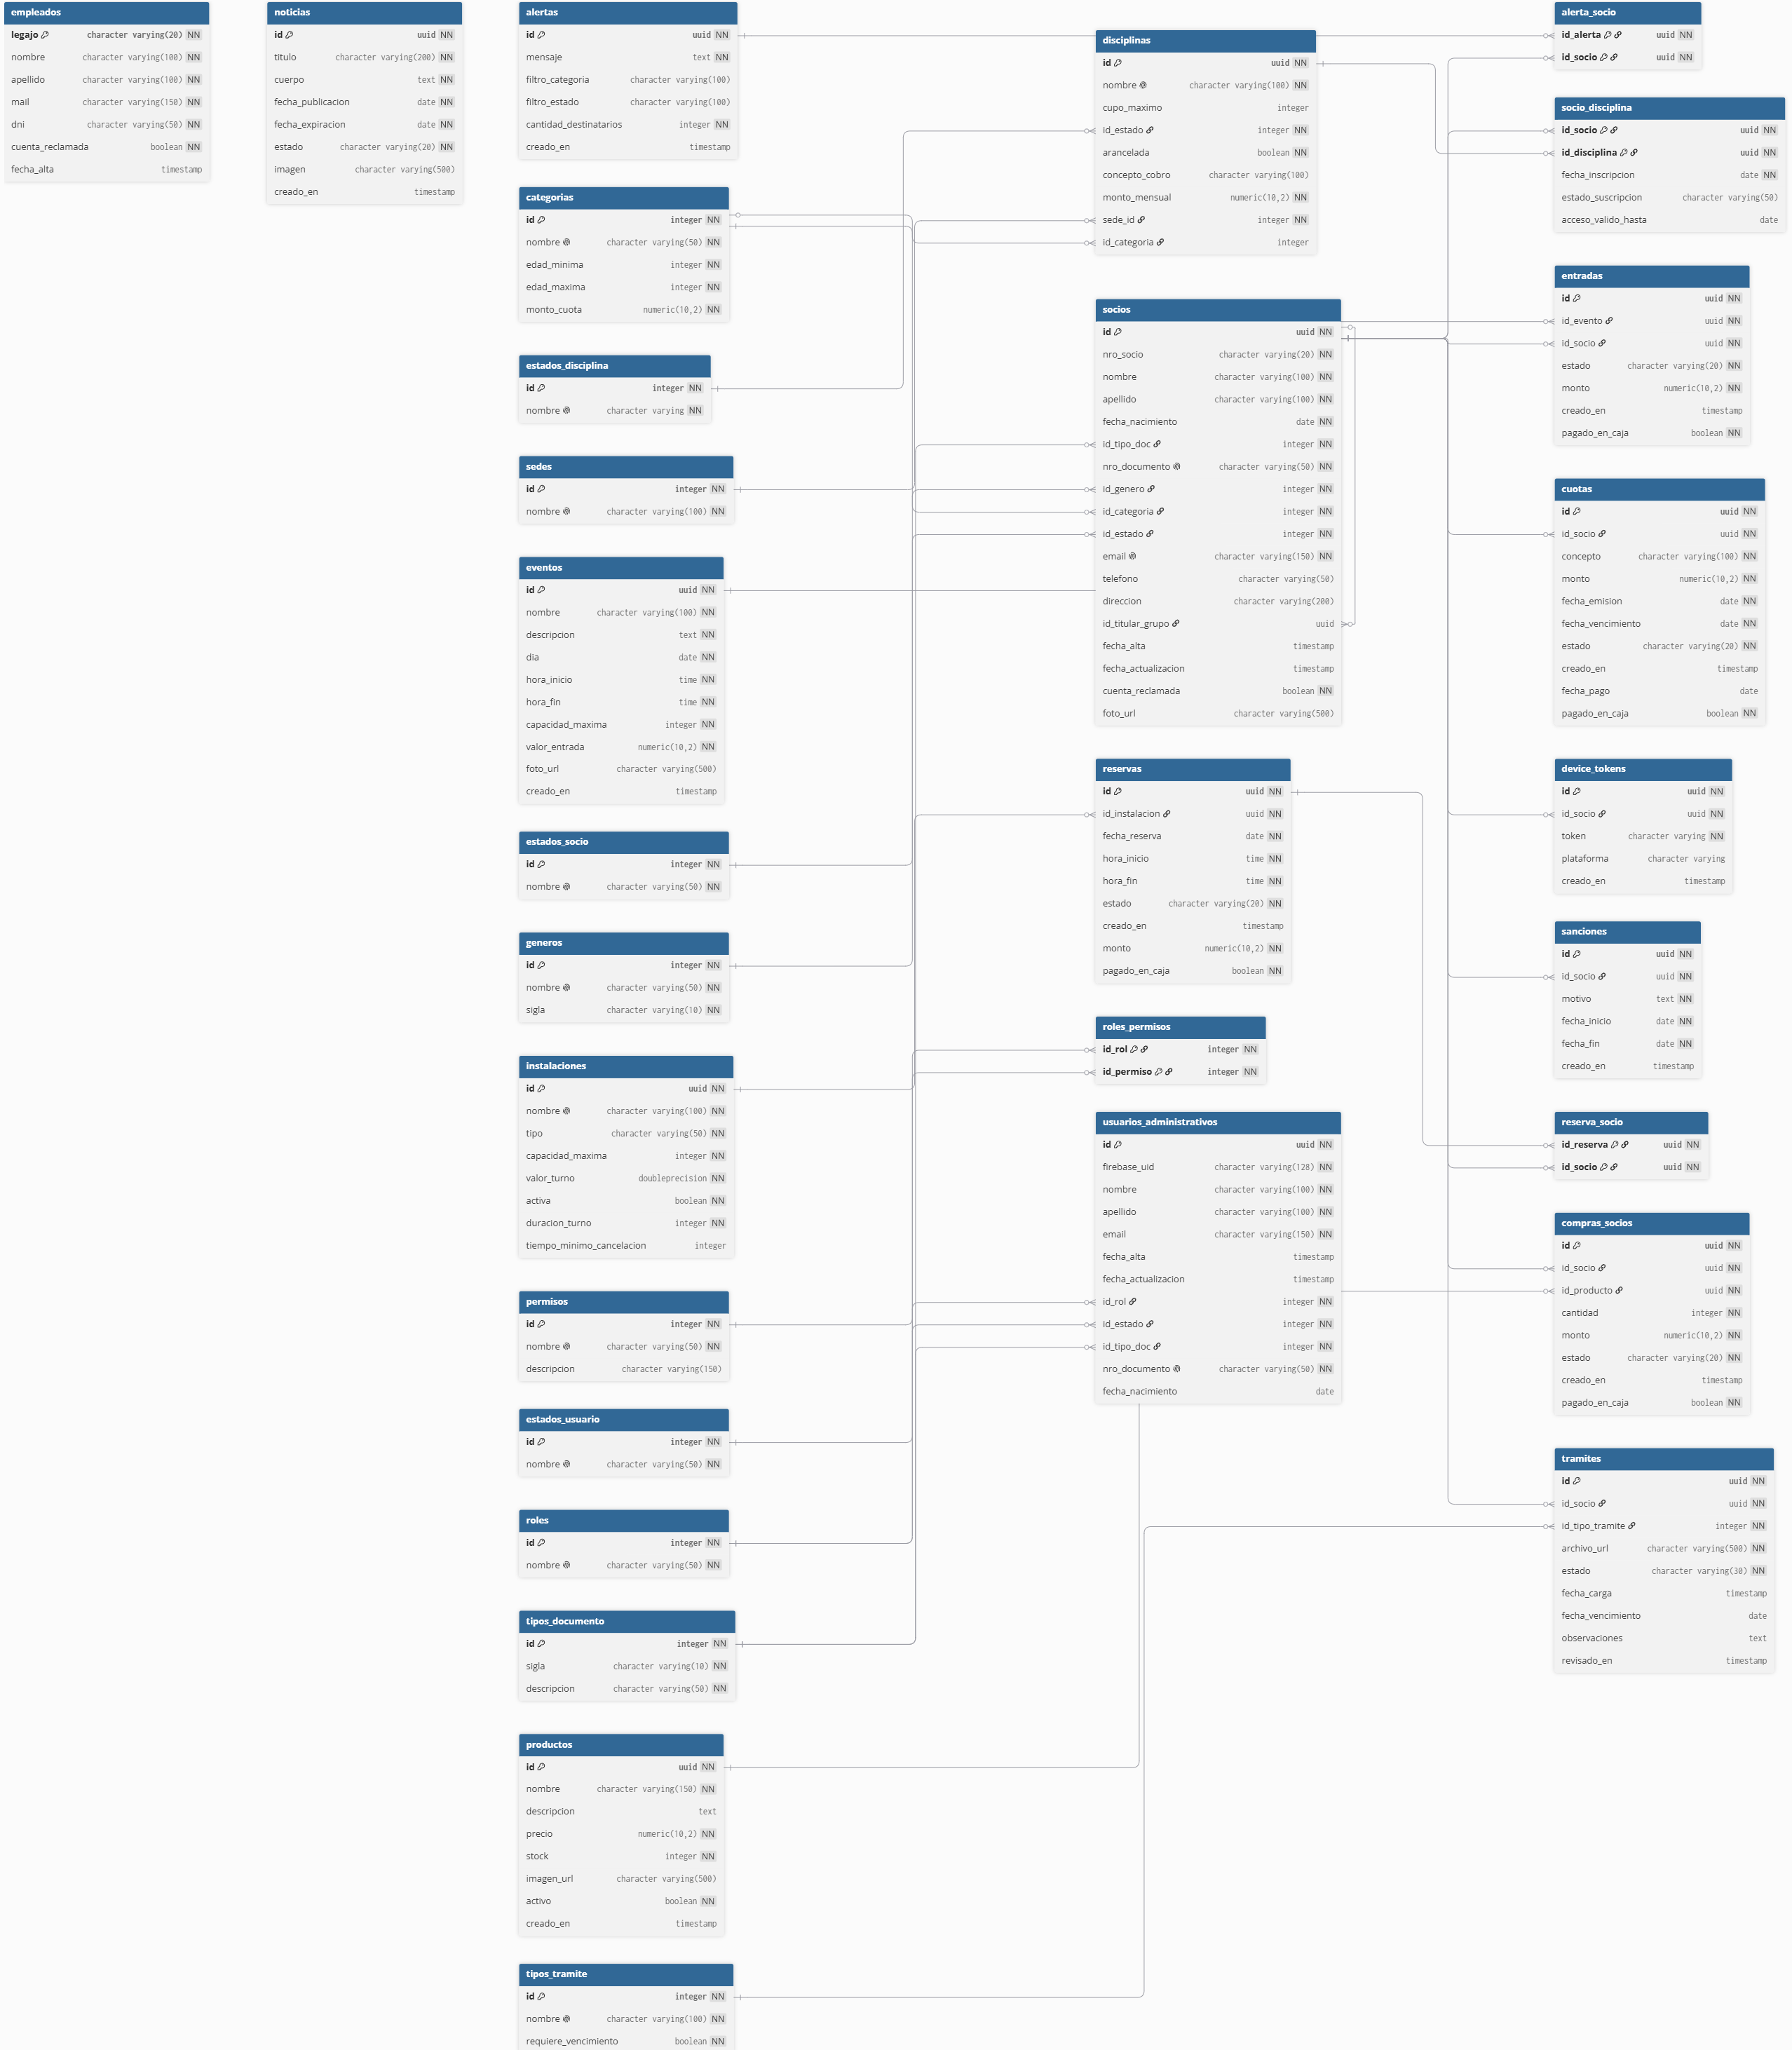
\includegraphics[width=0.85\textwidth]{img/der/MS Core - Database.png}
    \caption{Modelo lógico de datos encargado del control de identidad, categorías societarias y perfiles del padrón.}
    \label{fig:der_core}
\end{figure}

\newpage

\subsubsection{Base de datos de finanzas y facturación}
Esquema especializado en registrar transacciones monetarias. Controla los estados de las facturaciones mensuales, la generación de comprobantes, el historial de pagos efectuados y las firmas de integración con las pasarelas de pago digitales externas.

\begin{figure}[h!]
    \centering
    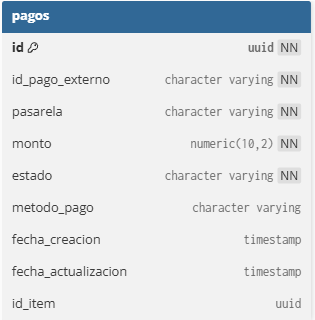
\includegraphics[width=0.6\textwidth]{img/der/MS Payments - Database.png}
    \caption{Modelo de persistencia para el control transaccional, vencimientos de cuotas y conciliación financiera.}
    \label{fig:der_payments}
\end{figure}

\subsubsection{Base de datos de analítica predictiva}
Modelo optimizado para la recopilación histórica de métricas de comportamiento e interacciones. Estructura los conjuntos de datos limpios necesarios para nutrir las tareas asíncronas y los algoritmos predictivos que alertan sobre posibles tendencias de morosidad.

\begin{figure}[h!]
    \centering
    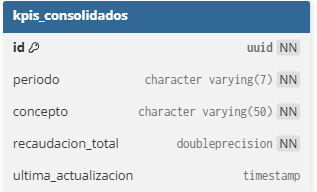
\includegraphics[width=0.6\textwidth]{img/der/MS Analytics & AI - Database.png}
    \caption{Almacenamiento estructurado para logs analíticos, métricas predictivas e históricos de entrenamiento de modelos.}
    \label{fig:der_analytics}
\end{figure}

\newpage

\subsubsection{Base de datos de acceso inteligente}
Esquema responsable de gestionar la validación matemática y el control de ingresos. Almacena de forma segura los secretos criptográficos (TOTP) de cada usuario y registra el historial detallado de accesos, estados y lectores utilizados en los puntos de control del club.

\begin{figure}[h!]
    \centering
    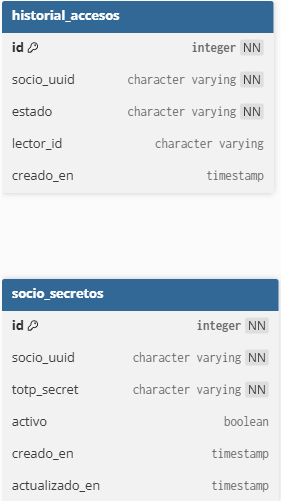
\includegraphics[width=0.7\textwidth]{img/der/Ms Acceso - Database.png}
    \caption{Modelo de persistencia para el registro de historial de accesos y administración de secretos TOTP.}
    \label{fig:der_acceso}
\end{figure}

\newpage

\subsection{Observabilidad y centralización de logs: Integración con Datadog}

Complementando de forma sinérgica las capacidades de inspección reactiva y proactiva del \textbf{Servicio de Healthchecker}, la plataforma \textbf{SocioUnido} incorpora \textbf{Datadog} como pilar central de su estrategia de observabilidad corporativa. En una arquitectura orientada a microservicios donde las transacciones involucran la interacción secuencial de múltiples nodos descentralizados (tales como la pasarela de API, los servicios de autenticación, el microservicio central y las pasarelas de pago externas), la dispersión y el aislamiento de los registros de ejecución (\textit{logs}) representan un desafío crítico para el diagnóstico de fallas y el análisis de rendimiento. 

La adopción de Datadog resuelve esta problemática actuando como una plataforma unificada de agregación, correlación y análisis de datos en tiempo real, sirviendo como una herramienta indispensable en todas las etapas del ciclo de vida del software, con especial énfasis en las fases de desarrollo activo, pruebas integrales automatizadas y monitoreo continuo del ecosistema.

\subsubsection{Ejes fundamentales de la implementación y casos de uso}

El despliegue y la configuración de esta solución de telemetría transversal abarca las siguientes dimensiones técnico-arquitectónicas:

\begin{itemize}
    \item \textbf{Agregación y centralización de logs heterogéneos:} Cada uno de los componentes del ecosistema de \textbf{SocioUnido} (los microservicios en sus respectivos contenedores, el API Gateway basado en KrakenD, y los motores de persistencia de datos) exporta sus flujos de salida estándar (\texttt{stdout} y \texttt{stderr}) de forma estructurada (típicamente en formato JSON). Datadog recolecta e indexa estos flujos de manera unificada, permitiendo al equipo de desarrollo realizar búsquedas transversales, filtrar por nivel de criticidad (\texttt{INFO}, \texttt{WARN}, \texttt{ERROR}) y reconstruir cronologías exactas de eventos sin necesidad de acceder de forma aislada a la infraestructura subyacente.
    
    \item \textbf{Trazabilidad distribuida y soporte para pruebas End-to-End (E2E):} Durante la ejecución de pruebas integrales o la simulación de flujos críticos del usuario final (por ejemplo, el login de un socio desde la PWA, pasando por la validación de identidad en el componente de autenticación hasta la confirmación de la pasarela de pagos), Datadog asocia un identificador único de traza (\textit{Trace ID}) a la petición a través de mecanismos de APM (\textit{Application Performance Monitoring}). Esta capacidad correlaciona los logs individuales de los distintos microservicios intervinientes en dicha transacción. Como resultado, es posible visualizar gráficamente el ciclo de vida completo de la solicitud, aislar cuellos de botella latentes y detectar con precisión milimétrica en qué punto exacto de la topología distribuida se originó una excepción.
    
    \item \textbf{Configuración de alertas proactivas para el ciclo de desarrollo:} Lejos de limitarse a un rol pasivo de auditoría \textit{post-mortem}, la plataforma ha sido configurada con monitores inteligentes que evalúan de forma continua las métricas de ingesta. Mediante reglas basadas en lógica condicional, el sistema dispara alertas inmediatas ante anomalías tales como picos inusuales en la tasa de errores HTTP 5xx, excepciones no controladas en el microservicio de analítica e inteligencia artificial, o degradaciones de latencia en la lógica de validación por TOTP del microservicio de acceso inteligente. Estas notificaciones tempranas optimizan los tiempos de depuración en entornos de desarrollo y control de calidad (\textit{QA}), previniendo el avance de regresiones hacia etapas posteriores del pipeline.
    
    \item \textbf{Visualización y análisis del comportamiento del sistema (\textit{Dashboards}):} Se podrían diseñar tableros de control personalizados que consoliden las métricas operativas y de negocio más relevantes de la plataforma. Estos páneles interactivos ofrecen una representación visual intuitiva de la salud del sistema, permitiendo realizar análisis tendenciales de la carga de trabajo, observar los patrones de tráfico concurrentes y evaluar la estabilidad de las integraciones con webhooks externos (como la API de WhatsApp). Esta visibilidad continua facilita la toma de decisiones basada en datos para el refinamiento de la arquitectura y la planificación de la escalabilidad.
\end{itemize}
